\chapter{Methodology }
\label{Methodology}
In previous chapters we introduced our research problem, listed and explained the solution options with the theoretical background. In this chapter we explain our practical approach for carrying out the research along with the software development required to support the experimentation and data analysis for our research. Following is the list of major tasks for the practical part of our research.
\begin{itemize}
\item Understanding energy efficiency, smart grids and available data.
\item Requirement engineering and use case preparation.
\item Understanding Data Analytics ecosystem, evaluating the Big Data tools and solutions.
\item Exploratory data analysis and selection of algorithms and data analysis tools with respect to use cases. 
\item Development of an end-to-end Big Data analytics platform.
\item Data collection, storage and preprocessing.
\item Use case specific data analysis and evaluation of the results.
\item Visualisation of the results 
\item Documentation of the research, process, software development and results.
\end{itemize}
Some of these tasks were required to be performed in a sequential way e.g. requirement engineering and evaluation of Big Data tools were required before developing the Big Data analytics platform or selecting the algorithms. Similarly we needed results before visualisations could be created. On the other hand some of the tasks could have been executed in parallel. For example the documentation was an ongoing process along with all other tasks. Similarly the literature review for understanding each component of our research was also an ongoing process. Then the iterations were required for continuous improvement.

To tackle these challenges, we needed a methodology that could support sequential and parallel task execution with support for iterations to improve. Like most of scientific research, fail fast and small to move ahead for success was the key for us. Most of the tasks required conceptualization and rapid prototyping. Taking it as a software development task initially, we had some candidate models such as the water fall model, the agile development model, the spiral model and the incremental model etc. Here we shall briefly discuss the advantages and disadvantages in context to our research project. 
\begin{itemize}
\item \textbf{ The waterfall model} offered the simplest approach to requirement engineering, design, implement, test and operate our research. However, it is inherently sequential and had weak support for iterations \cite{Laplante}.
\item \textbf{The agile development model} Agile methodology \cite{martin2003agile} is rapid, iterative and supports quick prototyping but it requires additional communication and management overhead like scrum meetings. Managing it along with stakeholders like VTT and the CIVIS projects was very hard.
\item \textbf{The spiral Model} is a risk driven process model. It supports prototyping, provides a good way of avoiding major failure risks, and it is iterative \cite{Boehm}. However, it needs a lot of resources during the planning phase especially when the spiral keeps growing in size. It is usually very successful for large projects but it has overheads for small projects like our thesis research. We shall be discussing more about using parts of the spiral model later in this chapter.
\item \textbf{The incremental model} relies on small incremental steps with each step consisting of independent design, implementation and testing phases \cite{jacobson1999unified}. In the beginning, incremental model was the best fit among other candidate models. We were able to prototype small functional units of the Big Data analytics platform very quickly while independently working on the use cases. However during the platform development and data analyses parts it created integration overheads. For example by integrating two different data processing tools together for a single use case, it becomes difficult when they were configured in two different incremental steps.  
\end{itemize}
Learning from the problems that we had faced while using incremental model, we altered our approach to an adapted version of another very flexible software research and development methodology known as ``Kumiega-Van Vliet Trading System Development Methodology''\cite{kumiega2008software}.

\section{Kumiega-Van Vliet model}\label{kvvm}   
      
The Kumiega-Van Vliet Trading System Development Methodology \((K|V)\) was developed in 2008 for software development required specifically for trading systems. It is the combination of three general purpose software and new product development models i.e. the waterfall model, the spiral model and the stage gate model. We have already explained the waterfall and spiral models. The stage gate model consists of stages e.g. scoping, development, implementation, testing etc. Each stage or combination of stages can be controlled with an approval gate. The process can not move from a stage to another stage if the gate in between them is not approved.This model provides a good control over the development model to ensure quality. However it may cause delays because of the organizational hierarchies dictating the gates.

 The \((K|V)\) model tries to overcome the short comings of the three models by combining them to a single paradigm for trading system development \cite{kumiega2008software}. In the spiral model, the spirals are divided into four basic steps i.e. research, planning, implementation and test. These four steps can be performed again and again in cycles. To avoid spirals  growing too much after each cycle, a stage gate controls if a process can pass to next stage or if it needs to be sent back to perform another cycle in the same stage. Just like the waterfall model, there can be number of stages. However, unlike the traditional waterfall model, in this model we have an an iteration channel for continuous improvement.

 \section{Adaptation of the Kumiega- Van Vliet model}\label{adaptation}
 The \((K|V)\) model is designed for software research  and development in the domain of financial services. With the built in stage gate controls, it requires some scale of hierarchical organizational structure to support the model. For our highly academic research case we have made certain adjustments. The most notable adaptation was to use deliverables and team reviews of respective deliverables as the main control for moving from one stage to the next stage instead of stage gate approvals. The concept of stages like the waterfall model helped in keeping our focus on the solutions for our problem statement. The spiral model cycles enabled us to iterate within a stage and improve the deliverables quality. Typically the decision of additional cycles was based on the feedback during the team review sessions. The inter-stage iteration channels helped us in improving our overall quality. The lessons learnt or the new directions identified during one iteration were included in the scope for the next iteration. It also allowed us to include supplementary topics in our scope without losing focus on mandatory issues.
 
 In our approach, we have divided the complete scope of research in four basic stages. Within each stage we had four steps. These intra-stage steps were different for each stage. These steps were corresponding to the main tasks that we discussed in the beginning of this chapter. A typical intra stage cycle ended with a set of deliverables. The deliverables were reviewed in a team review session. If required, the other stockholders such as VTT, were also involved in some of the review meetings. We shall be discussing it in detail when we describe our stage wise proceedings. At the end of each review session a decision was made to either move to next stage or try to improve via an additional cycle. Using all four intra-stage steps for additional cycles was not a must. This was another minor adaptation to the \((K|V)\) model. Similarly iterations were mostly initiated after stage three. There were three major iterations. During the iterations change of deliverables were not mandatory. However in practice it was observed that each iteration had caused some major or minor changes in stage deliverables. Having a small and informal team structure reduced our management and communication overheads. This also helped in rapid processing during iterations. Figure~\ref{fig:kv} illustrates our approach with the adapted version of \((K|V)\) model. Stage by stage description of our methodology is explained in the next section.   
 \begin{figure}[!h]
   \begin{center}
     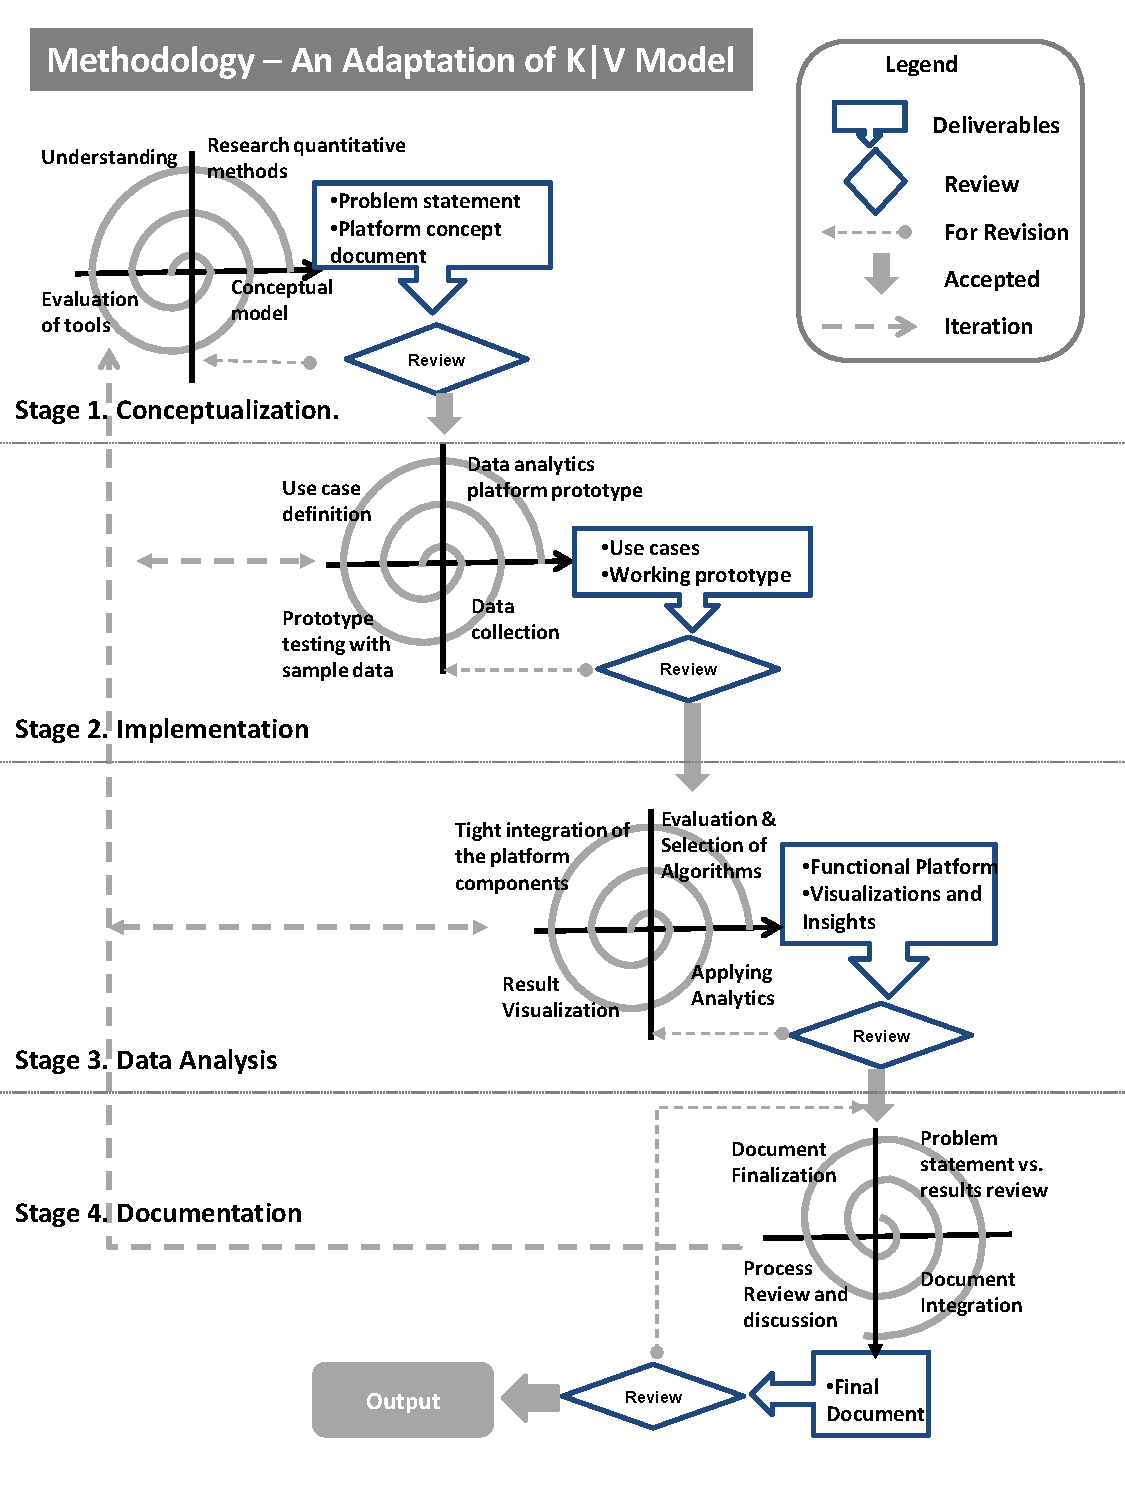
\includegraphics[width=\textwidth]{images/kv_method.pdf}
     \caption{Methodology, An Adaptation of \(K|V\) Model}
     \label{fig:kv}
   \end{center}
 \end{figure} 
\section{Stages, steps and cycles}\label{stages} 
We have already mentioned that there were four stages with each having four respective steps. Each stage was controlled via deliverables review sessions in a stage gate manner. While inside a stage, steps were executed in spiral cycles. The first cycle of the spiral had to pass through the four steps. The additional cycles were initiated if the further improvements were decided for deliverables in review session. All four steps were not mandatory for additional cycles. In this section we list and describe the stages along with the respective steps. We highlight some major cycles and deliverables. However the iterations will be discussed in the following section. Figure ~\ref{fig:kv} will be our main reference throughout this section. In this section we mention some functional components of our project e.g. logical architecture, data processing tools and algorithms. 
\subsection{Stage 1. Conceptualization } \label{concept}
At the start, our research problem was mainly concerned about processing the large volumes of the data coming from smart metering devices and understand the consumption patterns. So the primary focus of the conceptualisation stage was to describe our problem in detail, to understand important factors related to it, find and evaluate methods and tools to solve the problem. This stage had the following four steps.
\subsubsection{Step 1. Understanding} 
From the beginning, our research had two focus areas i.e. energy consumption and Big Data . The main purpose of this step was to understand important concepts related to these topics. Following were some main activities performed during this step:
\begin{itemize}
\item Intensive literature review.
\item Participation in CIVIS project Helsinki- Use case workshop 26-27 January 2014. It gave good insights about ecological and social factors effecting energy production, distribution and consumption.
\item Participation in VTT's Green Campus initiative introduction session.
\item Discussions and informal interviews with VTT's project lead for Green Campus Initiative.
\item Aalto University courses.
	\begin{enumerate}
	    \item Scalable Cloud Computing, as a good introduction to parallel batch processing and its uses for Big Data processing.
	    \item Information Visualisation, as an introduction to effective communication through data visualisation.
	  \end{enumerate}      
\end{itemize}

Literature review had been a constant step through out this stage, its cycles, and the iterations it went through.
\subsubsection{Step 2. Research quantitative methods} \label{qm}
This step involved finding and evaluating the various quantitative methods used for measuring energy consumption and benchmarking energy efficiency. Data aggregation methods like daily, monthly consumption, and average consumption were evaluated. Identification and theoretical evaluation of advanced analytical methods was also performed during this step.
\subsubsection{Step 3. Conceptual model}\label{cmodel}
This step was dedicated for finding available open source solutions to make a conceptual model for an end-to-end Big Data analytics. This step was mandatory for the deliverable of the Big Data platform concept paper. This step was also repeated during various iterations.

\subsubsection{Step 4. Evaluation of tools}
This step was in pair with \ref{cmodel}. All the tools listed in the conceptual model were tested during this step. A check-list of evaluated and selected tools was maintained. This list is available in Appendix\ref{chapter:first-appendixa}.

\subsubsection{Delivearbles of stage 1}
There were two deliverables of this stage
\begin{enumerate}
\item Problem Statement: First two steps of this stage were the main contributors for this deliverable.
\item Platform concept document. A document as result of step 3 and 4 of this stage. 
\end{enumerate}

\subsubsection{Stage 1 cycles}
In this stage we observed two cycles i.e. a cycle for producing the required deliverables and one additional cycle for the modification of platform concept document. The modification included changes in Big Data platform architecture and in ways of how to depict the conceptual model. Changes in architecture included additional components to handle data variety like MongoDB databases with Apache Pig. 

\subsection{Stage 2. Implementation}\label{implement}
This stage mainly includes requirement engineering and intensive software development to prototype and test the Big Data platform described in the concept paper as a deliverable from stage 1. This stage had the following four steps.
\subsubsection{Use case definition} \label{usecases}
In this step, based on the knowledge gained from stage 1. we decomposed our problem statement into lower level requirements that can be practically implemented using Big Data platform concept. Use cases went through several iterations. Details of iterations will be discussed later in section \ref{iteration}. However here we shall list the final list of use cases.
\begin{enumerate}
\item Understanding the seasonal energy usage patterns and their sensitivity with outside temperature.
\item Understanding characteristics of the buildings using daily energy consumption pattern.
\item Calculating the base load of the building to identify non user consumption of buildings
\item Classifying the buildings on the basis of the energy efficiency and analyse the seasonal shifts in this classification.
\item Predicting daily energy consumption of various household devices on the basis of previous consumption pattern.
\end{enumerate}
\subsubsection{Data analytics platform prototype}
This step involved the practical implementation of the platform concept. It covered installation, configuration, customization and integration of selected components as a proof of concept for an end-to-end Big Data platform that can collect, store, process, analyse and visualise data. Details of the components and implementation will be discussed in the next chapter.
\subsubsection{Data Collection}
As mentioned before, real life energy consumption data was provided by VTT. This data was collected by VTT from the smart metering devices installed on test sites. We had prepared our prototype platform to collect this from VTT data repositories continuously in real time. However due to some constraints we were not allowed to integrate our platform with VTT's data repositories. The data was provided to us initially via file transfer from a FTP\footnote{The File Transfer Protocol (FTP) is a standard network protocol used to transfer computer files from one host to another host over a TCP-based network, such as the Internet.} server. In the later stages, a websevice was opened for us to collect the data. The details of the data will be provided later in this document, however two types of data were collected during different iterations.
\begin{enumerate}
\item Hourly consumption of electricity, electricity used for heating, water, and reactive power in a set of buildings as part of VTT's Green Campus initiative.
\item Device level electricity consumption data of home appliances used in two apartments of Aalto Univerity campus residential housing blocks as test cases for VTT's Green Campus initiative.

\end{enumerate}
\subsubsection{Prototype testing with sample data}\label{prototype}
This step was only used during the first cycle of this stage and the first iteration of the whole process. The purpose of this stage was to test the full work flow from data collection to data visualisation using the developed prototype. The sample data was the randomly selected records from the hourly consumption data set. Although in this step we started with a smaller sample and then kept on increasing it. The complete data set was also tested. During this testing the following functionalities were tested.
\begin{enumerate}
\item Data collection.
\item Raw data storage.
\item Data cleaning to produce tidy data set.
\item Data pre-processing. Reducing the large data volume without losing insights. 
\item Storing pre-processed data into databases.
\item Testing of advanced analytics tools integrated within our prototype.
\item Data visualisation.  
\end{enumerate}
\subsubsection{Stage 2 deliverables}
The following were two deliverables of implementation stage.
\begin{enumerate}
\item Use case definition.
\item Working Prototype of Big Data platform concept.
\end{enumerate}
\subsubsection{Stage 2 cycles}
This stage went through two additional cycles on top of the first mandatory cycle. Within the two additional cycles, all the steps were performed except data collection. Data was collected only in the first cycle of this stage. 
The major revisions inside cycles included; alteration in use cases e.g. effect of external temperature on seasonal energy pattern was identified during one of the review sessions. Within prototype and protype testing the alterations were required to adapt for changes in use cases

\subsection{Stage 3 Data Analysis}
In this stage we used the data platform to analyse the collected data and produce the insights based on the use cases. We applied the basic and advanced analytics techniques introduced in the sections  \ref{daily}, \ref{seasonal}, \ref{classify}, \ref{predict}. This stage has the following four steps.
\subsubsection{Tight integration of the platform components}
In the section \ref{prototype} we tested all the units of the platform by manually enforcing the process i.e. taking out the  output of one module and manually feeding it to other module as the input. In this step we tried to automate the process by coupling the modules together in the form of a single process per use case. 
\subsubsection{Evaluation and selection of algorithms}\label{eval}
In this step we tried to find and compare various options of advanced analytics algorithms available for supporting our use cases. It involved quantitative methods considered in section \ref{qm}. However, the focus was more on the advanced analytics. The techniques explained in the sections; \ref{daily}, \ref{seasonal},  \ref{classify}, \ref{predict} were selected during this step. For evaluating the algorithms we were using samples from collected data as our training data. 
\subsubsection{Applying Analytics}
In this step we applied the selected algorithm on the complete data set. The insights generated from this step were the main results for our study. During the cycles of this stage, results from this step also affected the evaluation of algorithms in previous step, section \ref{eval}. Details related to this step will also explained in chapter \ref{chapter:Analysis}.    
\subsubsection{Result visualisation}
For ease of understanding the extracted insights in te previous step, We visualised the results in form of data graphs. Different tools for visualisations were used in this steps. Visualisation tools will be discussed in chapter \ref{chapter:platform}. For data visualisation we tried to implement the graphical practices discussed by Edward Tufte in his book ``The Visual Display of Quantitative Information'' \cite{tufte1983visual}.
\subsubsection{Stage 3 deliverables}
There were two deliverables of this stage.
\begin{enumerate}
\item Functional Platform. At the end of this stage, we had a fully functional platform capable of implementing the end-to-end data analytics.
\item Results and visualisation of the results. Providing required insight for the use cases. 
\end{enumerate}
\subsubsection{Stage 3 Cycles}
There were several cycles in this stage. However as deviation from our adaptation of the \((K|V)\) model, we just had one review session for this stage per iteration. Combination of different algorithms, their evaluation and then generating visualisations had to be repeated and tested many times. So reviewing in the intermediate cycles was very inefficient. This stage took more time because of many cycles and the wider spiral required to produce good quality results.
\subsection{Stage 4 Documentation}
Documentation was an ongoing process throughout the stages and the iterations. All of the stages had at least one deliverable in the form of some document e.g. stage 1 had the Big Data platform concept paper, stage 2 had the use cases document, in stage 3 we had data analysis and insights report. The purpose of the last stage was to consolidate all the information in different documents together in the shape of one single thesis report. The following were the four steps for this stage. 
\subsubsection{Problem statement vs. results review}\label{ps}
This step was the check for the consistency of our results with the research problem that we had in the beginning. We earlier mentioned that documentation stage was not always part of the iterations. However this stage was used during all the iterations to keep track of the main focal points, the complimentary and supplementary parts of our research.    
\subsubsection{Document Integration}
This step was concerned with the main task of this stage i.e. to consolidate the information together in the form of one consistent account. During this stage we tried to link the inter-stage documentation together along with theoretical background and the explanation of the process and the functional components of the project.
\subsubsection{Process Review and discussion}
The purpose of this step was to provide a retrospective view of the whole process. Also to highlight the main findings and discuss what could have been done better or more to improve the process and produce further results. This step also indicated some future directions for the relevant research areas. The considerations of this stage will be discussed further in chapter \ref{chapter:discussion}.
\subsubsection{Document Finalization}
This step controlled the final thesis report publishing aspects like formatting, sequencing of topics, proof reading and version control etc.  
\subsubsection{Stage 4 deliverables}
The final thesis report document was the mandatory deliverable  as the main output of the process and our research project. There were some supplementary deliverables like source codes, code books and procedures etc. that we intended to open source as part of our research.   
\subsubsection{Stage 4 Cycles}
to be written after the document reviews.
\section{Iterations} \label{iteration}
Iterative processes and work models do not require full specification right from beginning. Instead the implementation can start with a all part of specification. Then in a step wise approach the next scope is defined with consideration of lessons learnt and new directions found from previous iterations. This inherent characteristic of iterative processes had a vital role in our research. We started with a smaller scope i.e. two simple uses case. In earlier iteration we were able to focus on Big Data technologies and energy efficiency concepts more than the complex advanced analytics topics in later iterations. The findings and practical implementation in early phase enabled us to expand the scope later. We added more use cases with more focus on the data analysis and application of the Big Data for energy efficiency. Iterations also helped us in improving the quality of the research. 

In our approach, we went through 3 main iteration cycles. As mentioned in the section \ref{stages} each iteration did not involve the complete four stages and their respective steps. The first three stages were the main contributors in the iteration with step \ref{ps} of stage 4 as the main source for reviewing our proceedings against our targets. Table \ref{tab:iteration_table} lists the main activities in each iteration against the respective stages and steps.    

%\usepackage{lscape}
%\begin{landscape}
\begin{table}\tiny %[!t]
%\begin{sideways}
\begin{tabular}{|m{2.2cm}|>{\raggedright}m{1.7cm}|>{\raggedright}m{3.4cm}|>{\raggedright}m{3.4cm}|m{3.4cm}|}
\hline
	\textbf{Stages} & \textbf{Steps} & \textbf{Iteration 1} & \textbf{Iteration 2} & \textbf{Iteration 3} \\ \hline
	\multirow{4}{*}{\textbf{Conceptualization}} & Understanding  & Main Topics: Energy Efficiency, Eco-Efficiency, Demand Response, daily consumption, monthly consumption, smart grids, smart metering, NIALM, Big Data 3Vs, Parallel Batch Processing, MapReduce etc & Main Topics: Classification, clustering, K-means, Big Data Veracity and Valuation, Big Data Streaming, Lambda Architecture, Massively Parallel Processing etc. & Main Topics: Forecasting, Regression, Auto-regression, Moving Averages, ARIMA etc. \\ \cline{2-5}
	 & Research quantitative methods
 & Sampling, Aggregation,  Averages, Summation, standard deviation, distributions etc & Clustering,Centroid-based clustering; K-means, C-means, Distribution-based clustering; Cumulative distribution function,  Density-based clustering; DBSCAN.  & Time Series Analysis, Covariance, correlation, Regression, Auto-regression, Moving Averages, ARIMA, Random Forest etc. \\  \cline{2-5}
	 & Conceptual Model & Model for parallel batch processing & Massively Parallel processing added for faster processing & Additional Machine learning modules (Forecasting) \\  \cline{2-5}
	 & Evaluation of Tools & Apache; Hadoop, HDFS, Flume, Sqoop, oozie, Hive, Pig in Cloudera distribution.
R, mahout, Tableau, D3.JS  & Cloudera Impala, Spark, Hbase, MongoDB. & Weka, Cloudera Oryx,  R (Forecast package) \\ \hline
\multirow{4}{*}{\textbf{Implementation}} & Use case definition
 & List of use cases:
(1) Understanding the seasonal energy usage patterns and its sensitivity with outside temperature.
(2) Understanding characteristics of building using daily energy consumption pattern. & List of use cases:
(3) Calculate the base load of the building to identify non user consumption of buildings
(4) Classify building on basis of energy efficiency and analyse seasonal shifts in this classification. & (5) Predict daily energy consumption of various house hold devices on basis of previous consumption pattern. \\ \cline{2-5}
	 & Data analytics platform prototype
 & Parallel batch processing with capability to collect data from data from data servers and public social media streaming API s. Machine learning modules integration . Visualisation using Tableau Public. & Integration of on-line query engine with Cloudera Impala. This enabled near to real life Big Data processing. & Use of additional data mining and machine learning tools like Weka.  \\ \cline{2-5}
	 & Data collection
 & Hourly electricity and  electricity for heating consumption data from VTT's smart metering devices on pilot sites for Green Campus Initiative. & Device level electricity consumption data from VTT's NIALM devices installed in two selected residential apartments. & One month twitter data collection for Green Hackathon using collection of energy related keywords.  \\ \cline{2-5}
	 & Prototype testing with sample data
 & Testing with samples from hourly consumption data. Testing with complete hourly consumption data. & Testing with NIALM device data. & Testing the prediction model using NIALM device data an additional data mining and machine learning tools. Performance comparison between non parallel executing, parallel batch processing and Masively parallel processing tools. \\ \hline
	\multirow{4}{*}{\textbf{Data Analysis}}	 & Tight integration of the platform components
 & End-to-End workflow implementation i.e. from data collection, storage, preprocessing and analysis to visualisation of results. Limited to batch processing only & Integration of Impala.  &  \\ \cline{2-5}
	 & Evaluation \& Selection of Algorithms
 & Selected quantative methods: Basic aggregations e.g. averages , summations and groupings. & Selected quantative method: K-means clustering  & Selected quantative methods:  ARIMA, linear regression and Random Forest forecasting techniques. \\ \cline{2-5}
	 & Applying Analytics
 & Applying basic aggregations according to use case 1 and 2. & 1) Basic Aggregation for use case 3
2) K-means clustering for use case 4 & ARIMA and Random Forest algorithms for use case 5. \\ \cline{2-5}
	 & Result Visualisation
 & Using Tableau Public & Using Tableau Public  & Using R plots and Weka \\ \hline
\multirow{4}{*}{\textbf{Documentation}}	 & Problem statement vs. results review
 & Results for use case 1 and 2 reviewed. & Results for use case 3 and 4 reviewed. & Results for use case 5 reviewed. \\ \cline{2-5}
	 & Document Integration
 & Step not used  & Step not used  & Integration of  platform concept paper, data analysis report and use documentation.  \\ \cline{2-5}
	 & Process Review and discussion
 & Step not used  & Step not used  & Theoratical background explainations and linkages to research. Future directions for related work. \\ \cline{2-5}
	 & Document Finalization
 & Step not used  & Step not used  & Document formating. \\ \hline
\end{tabular}
%\end{sideways}
\caption{Details of the iterations}
\label{tab:iteration_table}
\end{table}
%\end{landscape} 